\section{Auswertung}
\label{sec:Auswertung}
In der folgenden Tabelle sind alle Messwerte aufgeführt
Die Temperaturverläufe sind in dem folgenden Diagramm dargestellt und mit einer
linearen Ausgleichstrechnung approximiert.
\subsection{Aufgabe. a}
\begin{figure}
  \centering
  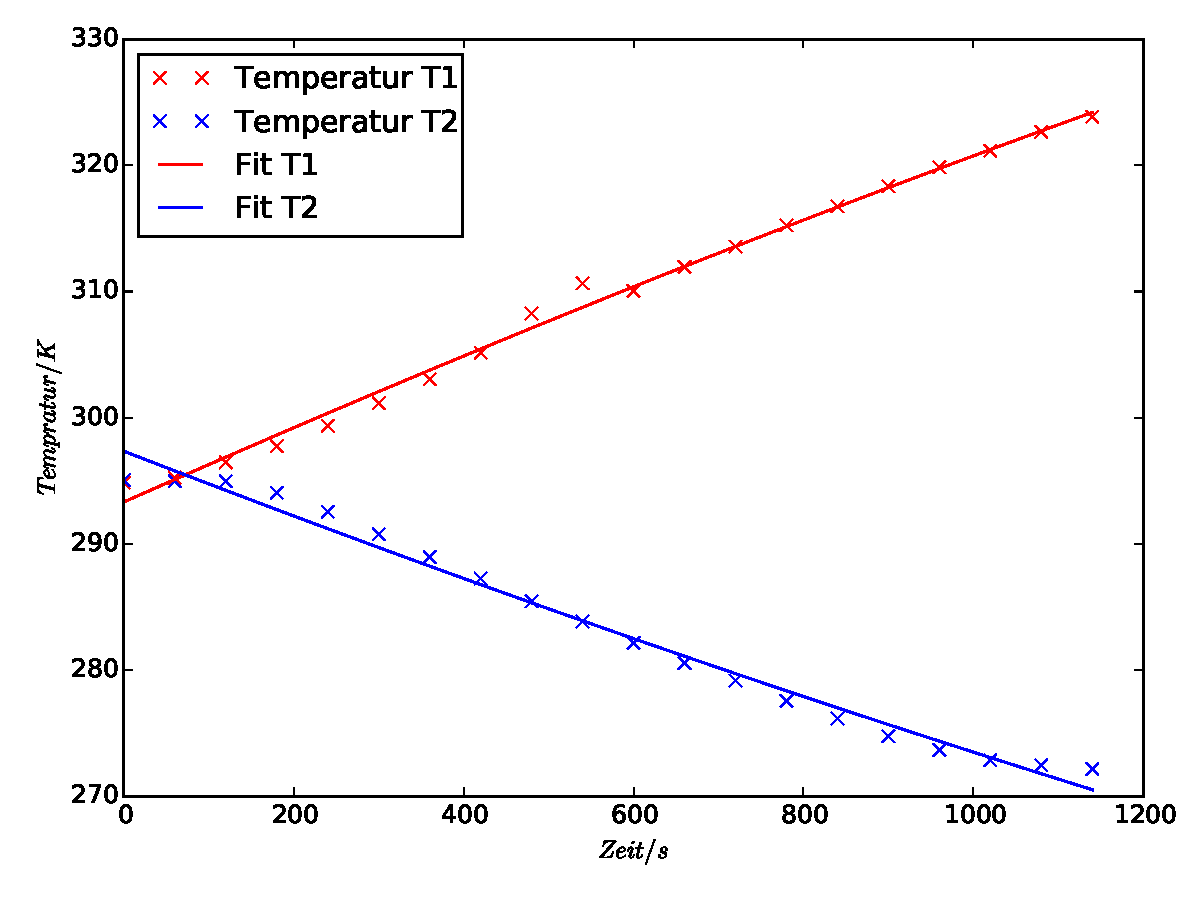
\includegraphics[width=0.60\textwidth]{Temperaturgraphik.pdf}
  \caption{Approximation des Temperaturverlaufes}
  \label{fig:Tempverlauf}
\end{figure}
Die Näherung wurde mit scientific Python gemacht und ist gegeben durch
\begin{equation}
  T(t)=At^2+Bt+C .
\end{equation}
Die Parameter für erwärmte Reservoir $T_1$ sind
\begin{equation}
  A=(  -0.000002485)\frac{K}{s^2}
  B=(   0.029925168)\frac{K}{s}
  C=( 293.312793014)K
\end{equation}
Die Parameter für den anderen Behälter$T_2$ sind
\begin{equation}
  A=(  0.000002259)\frac{K}{s^2}
  B=( -0.026112097)\frac{K}{s}
  C=(297.339350549)K

\end{equation}
